\chapter{Threads}

\section{Motivation for Threads}

Threads enable concurrent execution within a process. They improve responsiveness, resource sharing, scalability, and CPU utilization.

Benefits:

\begin{itemize}
\item Improved responsiveness
\item Better resource sharing
\item Lower overhead than processes
\item Efficient multicore utilization
\item Increased throughput
\end{itemize}

\begin{figure}[H]
\centering
\begin{tikzpicture}
\node[draw, rectangle] (p) {Process};
\node[draw, rectangle, below left=1cm and 1cm of p] (t1) {Thread 1};
\node[draw, rectangle, below=1cm of p] (t2) {Thread 2};
\node[draw, rectangle, below right=1cm and 1cm of p] (t3) {Thread 3};

\draw (p)--(t1);
\draw (p)--(t2);
\draw (p)--(t3);
\end{tikzpicture}
\caption{Multiple Threads Inside a Process}
\end{figure}

\section{What is a Thread}

A thread is the smallest unit of CPU execution.

Each thread contains:

\begin{itemize}
\item Program Counter
\item Register Set
\item Stack
\item Thread State
\end{itemize}

Shared among threads:

\begin{itemize}
\item Code Segment
\item Heap
\item Open Files
\item Global Variables
\end{itemize}

\section{Process vs Thread}

\begin{longtable}{|p{4cm}|p{5cm}|p{5cm}|}
\hline
Feature & Process & Thread \\
\hline
Address Space & Separate & Shared \\
\hline
Creation Cost & High & Low \\
\hline
Context Switch & Expensive & Cheaper \\
\hline
Communication & IPC Needed & Shared Memory \\
\hline
Isolation & Strong & Weak \\
\hline
Failure Impact & Isolated & Can Affect Process \\
\hline
\end{longtable}

\section{Thread States}

Typical thread states:

\begin{itemize}
\item New
\item Ready
\item Running
\item Waiting
\item Terminated
\end{itemize}

\begin{figure}[H]
\centering
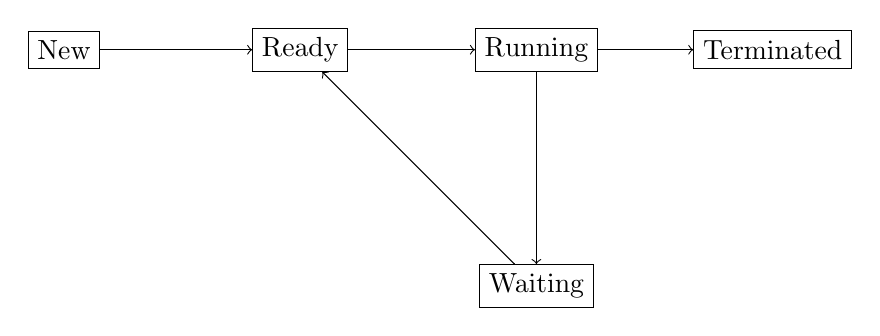
\begin{tikzpicture}
\node[draw] (new) at (0,0) {New};
\node[draw] (ready) at (3,0) {Ready};
\node[draw] (run) at (6,0) {Running};
\node[draw] (wait) at (6,-3) {Waiting};
\node[draw] (term) at (9,0) {Terminated};

\draw[->] (new)--(ready);
\draw[->] (ready)--(run);
\draw[->] (run)--(wait);
\draw[->] (wait)--(ready);
\draw[->] (run)--(term);
\end{tikzpicture}
\caption{Thread State Diagram}
\end{figure}

\section{User Threads}

User threads are managed entirely in user space.

Advantages:

\begin{itemize}
\item Fast creation
\item Fast switching
\item No kernel involvement
\end{itemize}

Disadvantages:

\begin{itemize}
\item Blocking system call blocks all threads
\item Limited multicore support
\end{itemize}

\section{Kernel Threads}

Kernel threads are managed by the operating system.

Advantages:

\begin{itemize}
\item True parallelism
\item Better scheduling
\item Blocking affects only one thread
\end{itemize}

Disadvantages:

\begin{itemize}
\item Higher overhead
\item More expensive context switches
\end{itemize}

\section{Multithreading Models}

Models define mapping between user threads and kernel threads.

\section{Many-to-One}

Multiple user threads mapped to a single kernel thread.

\begin{figure}[H]
\centering
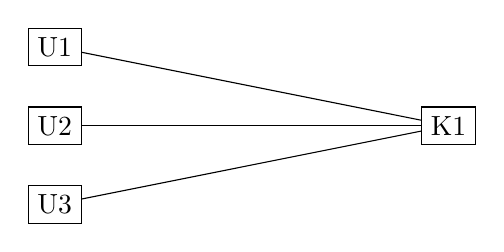
\begin{tikzpicture}
\node[draw] (u1) at (0,2) {U1};
\node[draw] (u2) at (0,1) {U2};
\node[draw] (u3) at (0,0) {U3};
\node[draw] (k1) at (5,1) {K1};

\draw (u1)--(k1);
\draw (u2)--(k1);
\draw (u3)--(k1);
\end{tikzpicture}
\caption{Many-to-One Model}
\end{figure}

Pros:
\begin{itemize}
\item Efficient
\end{itemize}

Cons:
\begin{itemize}
\item No parallel execution
\end{itemize}

\section{One-to-One}

Each user thread maps to one kernel thread.

\begin{figure}[H]
\centering
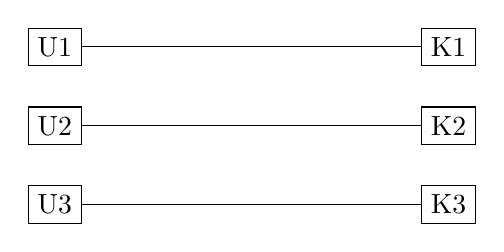
\begin{tikzpicture}
\node[draw] (u1) at (0,2) {U1};
\node[draw] (u2) at (0,1) {U2};
\node[draw] (u3) at (0,0) {U3};

\node[draw] (k1) at (5,2) {K1};
\node[draw] (k2) at (5,1) {K2};
\node[draw] (k3) at (5,0) {K3};

\draw (u1)--(k1);
\draw (u2)--(k2);
\draw (u3)--(k3);
\end{tikzpicture}
\caption{One-to-One Model}
\end{figure}

\section{Many-to-Many}

Many user threads mapped to many kernel threads.

\begin{figure}[H]
\centering
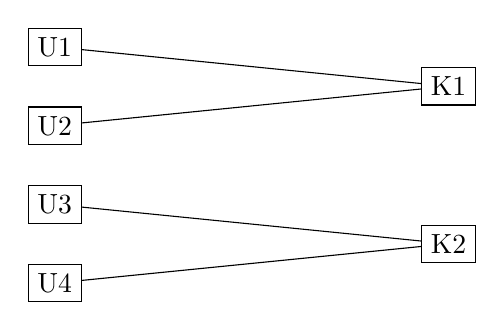
\begin{tikzpicture}
\node[draw] (u1) at (0,3) {U1};
\node[draw] (u2) at (0,2) {U2};
\node[draw] (u3) at (0,1) {U3};
\node[draw] (u4) at (0,0) {U4};

\node[draw] (k1) at (5,2.5) {K1};
\node[draw] (k2) at (5,0.5) {K2};

\draw (u1)--(k1);
\draw (u2)--(k1);
\draw (u3)--(k2);
\draw (u4)--(k2);
\end{tikzpicture}
\caption{Many-to-Many Model}
\end{figure}

\section{Thread Libraries}

Popular thread libraries:

\begin{itemize}
\item POSIX Threads (Pthreads)
\item Java Threads
\item Python threading module
\end{itemize}

\section{POSIX Threads}

\subsection{Pthreads Example}

\begin{lstlisting}[language=C,style=interviewcode]
#include <pthread.h>
#include <stdio.h>

void* work(void* arg) {
    printf("Hello Thread\n");
    return NULL;
}

int main() {
    pthread_t t;
    pthread_create(&t, NULL, work, NULL);
    pthread_join(t, NULL);
    return 0;
}
\end{lstlisting}

\section{Java Threads}

Java provides Thread class and Runnable interface.

\subsection{Java Example}

\begin{lstlisting}[language=Java,style=interviewcode]
class Worker extends Thread {
    public void run() {
        System.out.println("Running");
    }
}

public class Main {
    public static void main(String[] args) {
        Worker t = new Worker();
        t.start();
    }
}
\end{lstlisting}

\section{Python Threads}

Python provides the threading module.

\subsection{Python Example}

\begin{lstlisting}[language=Python,style=interviewcode]
import threading

def task():
    print("Thread running")

t = threading.Thread(target=task)
t.start()
t.join()
\end{lstlisting}

\section{Thread Pools}

Thread pools maintain a collection of reusable worker threads.

Advantages:

\begin{itemize}
\item Reduced creation overhead
\item Better resource management
\item Improved throughput
\item Controlled concurrency
\end{itemize}

\begin{figure}[H]
\centering
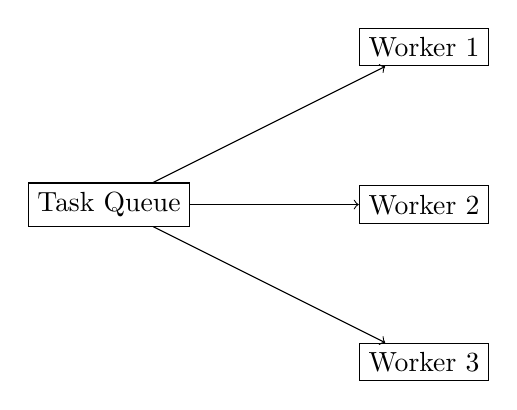
\begin{tikzpicture}
\node[draw] (queue) at (0,0) {Task Queue};

\node[draw] (t1) at (4,2) {Worker 1};
\node[draw] (t2) at (4,0) {Worker 2};
\node[draw] (t3) at (4,-2) {Worker 3};

\draw[->] (queue)--(t1);
\draw[->] (queue)--(t2);
\draw[->] (queue)--(t3);
\end{tikzpicture}
\caption{Thread Pool Architecture}
\end{figure}

\section{Thread Safety}

Thread-safe code behaves correctly when accessed concurrently.

Techniques:

\begin{itemize}
\item Mutexes
\item Semaphores
\item Read-Write Locks
\item Atomic Operations
\item Immutability
\end{itemize}

\section{Thread Local Storage}

Thread Local Storage (TLS) provides thread-specific variables.

Characteristics:

\begin{itemize}
\item Private to each thread
\item Prevents race conditions
\item Useful for caches and contexts
\end{itemize}

\section{Multicore Execution}

Multiple threads can execute simultaneously on different CPU cores.

\begin{figure}[H]
\centering
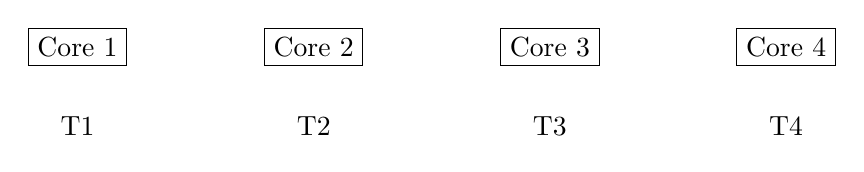
\begin{tikzpicture}
\node[draw] (c1) at (0,0) {Core 1};
\node[draw] (c2) at (3,0) {Core 2};
\node[draw] (c3) at (6,0) {Core 3};
\node[draw] (c4) at (9,0) {Core 4};

\node at (0,-1) {T1};
\node at (3,-1) {T2};
\node at (6,-1) {T3};
\node at (9,-1) {T4};
\end{tikzpicture}
\caption{Parallel Execution on Multiple Cores}
\end{figure}

\section{Interview Notes}

\begin{itemize}
\item Threads share address space; processes do not.
\item Context switching between threads is cheaper.
\item Thread pools improve scalability.
\item Kernel threads enable true parallelism.
\item Thread safety is critical in concurrent systems.
\item TLS provides per-thread data storage.
\end{itemize}

\section{Key Takeaways}

\begin{keytakeaways}
Threads are lightweight execution units within a process. They share memory and resources, enabling efficient concurrency. User threads are fast but limited, while kernel threads provide true parallelism. Multithreading models define mappings between user and kernel threads. Thread pools improve performance. Thread safety prevents race conditions. Thread Local Storage provides private per-thread data. Multicore systems allow simultaneous execution of multiple threads.
\end{keytakeaways}

\section{Interview Questions with Answers}

\begin{enumerate}
\item What is a thread?\\
Smallest schedulable unit of execution.

\item What resources are shared among threads?\\
Code, heap, files, globals.

\item What resources are private to a thread?\\
Stack, registers, PC.

\item Process vs thread?\\
Threads share memory; processes do not.

\item Why use threads?\\
Concurrency and responsiveness.

\item What is thread safety?\\
Correct behavior under concurrent access.

\item What is a race condition?\\
Unexpected behavior due to unsynchronized access.

\item What is TLS?\\
Thread-specific storage.

\item What is a thread pool?\\
Reusable collection of worker threads.

\item Advantage of thread pools?\\
Lower creation overhead.

\item What is a user thread?\\
Managed in user space.

\item What is a kernel thread?\\
Managed by OS kernel.

\item Many-to-One model?\\
Many user threads to one kernel thread.

\item One-to-One model?\\
One user thread to one kernel thread.

\item Many-to-Many model?\\
Many user threads to many kernel threads.

\item Why are threads lightweight?\\
Shared address space.

\item What is context switching?\\
Switching CPU execution between threads.

\item Can threads run in parallel?\\
Yes on multicore systems.

\item What is pthreads?\\
POSIX thread API.

\item Why synchronize threads?\\
Prevent data corruption.
\end{enumerate}

\section{MCQs with Answers}

\begin{enumerate}
\item Smallest execution unit?
\begin{enumerate}[label=(\alph*)]
\item Process
\item Thread
\item File
\item Socket
\end{enumerate}
Answer: (b)

\item Threads share:
\begin{enumerate}[label=(\alph*)]
\item Stack
\item Registers
\item Heap
\item PC
\end{enumerate}
Answer: (c)

\item Private to a thread:
\begin{enumerate}[label=(\alph*)]
\item Heap
\item Code
\item Stack
\item Files
\end{enumerate}
Answer: (c)

\item Thread creation cost is:
\begin{enumerate}[label=(\alph*)]
\item High
\item Low
\item Infinite
\item None
\end{enumerate}
Answer: (b)

\item User threads are managed by:
\begin{enumerate}[label=(\alph*)]
\item Kernel
\item Hardware
\item Library
\item BIOS
\end{enumerate}
Answer: (c)

\item Kernel threads are managed by:
\begin{enumerate}[label=(\alph*)]
\item OS
\item Compiler
\item JVM
\item Loader
\end{enumerate}
Answer: (a)

\item Many-to-One supports:
\begin{enumerate}[label=(\alph*)]
\item Full parallelism
\item No parallelism
\item NUMA
\item DMA
\end{enumerate}
Answer: (b)

\item Thread pool purpose:
\begin{enumerate}[label=(\alph*)]
\item Reduce overhead
\item Increase RAM
\item Reduce Disk
\item Increase Cache
\end{enumerate}
Answer: (a)

\item TLS stands for:
\begin{enumerate}[label=(\alph*)]
\item Thread Local Storage
\item Thread Lock Service
\item Task Local Store
\item Thread Layer Storage
\end{enumerate}
Answer: (a)

\item Java thread starts with:
\begin{enumerate}[label=(\alph*)]
\item run()
\item start()
\item create()
\item init()
\end{enumerate}
Answer: (b)

\item Pthreads is:
\begin{enumerate}[label=(\alph*)]
\item Java API
\item POSIX API
\item Python API
\item DB API
\end{enumerate}
Answer: (b)

\item Thread safety prevents:
\begin{enumerate}[label=(\alph*)]
\item Caching
\item Scheduling
\item Race Conditions
\item Paging
\end{enumerate}
Answer: (c)

\item Context switch between threads is:
\begin{enumerate}[label=(\alph*)]
\item Expensive
\item Cheaper
\item Impossible
\item Random
\end{enumerate}
Answer: (b)

\item Multicore systems enable:
\begin{enumerate}[label=(\alph*)]
\item Parallelism
\item Deadlock
\item Paging
\item Segmentation
\end{enumerate}
Answer: (a)

\item Shared memory enables:
\begin{enumerate}[label=(\alph*)]
\item Easy communication
\item Slow execution
\item Paging
\item Swapping
\end{enumerate}
Answer: (a)

\item One-to-One maps:
\begin{enumerate}[label=(\alph*)]
\item Many U to One K
\item One U to One K
\item Many U to Many K
\item One U to Many K
\end{enumerate}
Answer: (b)

\item Running thread state:
\begin{enumerate}[label=(\alph*)]
\item Executing on CPU
\item Waiting for CPU
\item Created
\item Destroyed
\end{enumerate}
Answer: (a)

\item Waiting state means:
\begin{enumerate}[label=(\alph*)]
\item Finished
\item Blocked
\item Created
\item Deleted
\end{enumerate}
Answer: (b)

\item Thread library example:
\begin{enumerate}[label=(\alph*)]
\item Pthreads
\item DNS
\item HTTP
\item BIOS
\end{enumerate}
Answer: (a)

\item Threads primarily improve:
\begin{enumerate}[label=(\alph*)]
\item Concurrency
\item Storage
\item Disk Size
\item Network Speed
\end{enumerate}
Answer: (a)
\end{enumerate}

\section{Revision Notes}

\begin{revisionnotes}
\item Threads are lightweight execution units.
\item Threads share process resources.
\item Stack and registers are thread-private.
\item User threads are fast but limited.
\item Kernel threads support parallelism.
\item Many-to-One limits concurrency.
\item One-to-One is widely used.
\item Many-to-Many is scalable.
\item Thread pools reduce overhead.
\item Thread safety prevents races.
\item Synchronization protects shared data.
\item TLS provides thread-specific variables.
\item Multicore processors enable true parallel execution.
\item Pthreads are POSIX compliant.
\item Java and Python provide built-in thread support.
\end{revisionnotes}

\section{Cheat Sheet}

\begin{longtable}{|p{5cm}|p{8cm}|}
\hline
Concept & Summary \\
\hline
Thread & Smallest execution unit \\
\hline
Shared Resources & Heap, code, files \\
\hline
Private Resources & Stack, registers, PC \\
\hline
User Thread & Managed in user space \\
\hline
Kernel Thread & Managed by OS \\
\hline
Many-to-One & Many U $\rightarrow$ One K \\
\hline
One-to-One & One U $\rightarrow$ One K \\
\hline
Many-to-Many & Many U $\rightarrow$ Many K \\
\hline
Pthreads & POSIX threading API \\
\hline
Thread Pool & Reusable worker threads \\
\hline
Thread Safety & Correct concurrent behavior \\
\hline
TLS & Thread-specific data \\
\hline
Race Condition & Unsynchronized shared access \\
\hline
Multicore & Parallel thread execution \\
\hline
Context Switch & CPU switches execution \\
\hline
\end{longtable}